\documentclass{article}

\usepackage[cm]{fullpage}
\usepackage{graphicx,wrapfig}
\usepackage{float}
\usepackage{amsmath, mathrsfs,amssymb}
\usepackage{verbatim}
\usepackage[margin=.5in]{geometry}
\usepackage{caption}
\usepackage{subcaption}
\usepackage{enumitem}
\usepackage{amsmath}
\numberwithin{equation}{section}

\usepackage{multicol}
\usepackage{lipsum}
\usepackage{capt-of}
\usepackage{dsfont}

\usepackage[pdftex,pagebackref=true]{hyperref}
\usepackage[svgnames,dvipsnames,x11names]{xcolor}
\hypersetup{
colorlinks,%
linkcolor=RoyalBlue2,  % colour of links to eqns, tables, sections, etc
urlcolor=Sienna4,   % colour of unboxed URLs
citecolor=RoyalBlue2  % colour of citations linked in text
}

\usepackage{sectsty}
\sectionfont{\large}

\def\ci{\perp\!\!\!\perp}   

\title{663 Final Project Progress Report}
\author{Jake Coleman and Sayan Patra}
\date{}
\begin{document}
\maketitle

\section{Abstract}
For our project we will use Neal's 2011 paper, ``MCMC using Hamiltonian dynamics." The paper discusses how to use Hamiltonian dynamics as a sampling scheme to explore target spaces better than traditional Metropolis-Hastings algorithms. The Hamiltonian is the sum of potential energy (based on position) and kinetic energy (based on momentum) - Hamilton's equations relate the two partial derivatives of the Hamiltonian to each other, and define a mapping from the state at time $t$ to the state at time $t + s$. In Hamiltonian Monte Carlo (HMC), we draw auxiliary momentum variables from a Gaussian distribution, and use Hamiltonian dynamics simulations to update the position variable (which follows the distribution of interest). At the end of a user-defined number of steps of simulation, the new variables are accepted or rejected in a Metropolis-Hastings step.\\

In this report we will explore basic HMC with the ``Leapfrog'' discretization method, and follow some examples (such as highly-correlated multivariate Gaussian distributions) comparing HMC to random-walk Metropolis Hastings that show improvement for HMC. We will establish the superiority of the HMC method over regular random walk sampling schemes in the case of higher dimensions. We will also implement an extension of HMC proposed by Neal (1994) that uses ``windows'' of states to allow for a high probability of acceptance for all trajectories. Finally, we plan on converting the code to Cython or JIT to speed up implementation, and compare to existing HMC packages.

\section{Introduction}
Markov Chain Monte Carlo (MCMC) has been used to simulate distributions since the landmark paper by Metropolis et al. (1953). In this report we follow Neal (2011) in his exploration of Hamiltonian Monte Carlo (HMC), a variant of MCMC which utilizes properties physical properties of molecules known as ``\textit{Hamiltonian dynamics}.'' Hamiltonian dynamics rely on deterministic motion of molecules described by Newton's laws of motion, and were only applied as part of an MCMC algorithm in 1987 by Duane, Kennedy, Pendleton, and Roweth, with statistically applications beginning in 1996 with Neal's paper on neural networks.  The marriage of deterministic molecular simulations and MCMC allows fast exploration of state spaces of distributions while avoiding random walks necessary in Metropolis-Hasting algorithms.\\

In the subsequent sections we describe the Hamiltonian dynamics (section $3$) and how to construct a MCMC method using them (section $4$). Like in other Markov Chain methods HMC has its issues of tuning, which are discussed briefly in section $4$. Section $5$ compares HMC to Metropolis random-walk, in both low and high dimensions. In section $6$ a variation of HMC is presented, where the acceptance rate of HMC is shown to be increased by looking at the ``windows" of states at the beginning and the end of the trajectories.


\section{Background - Hamiltonian Dynamics}
Hamiltonian dynamics describes the potential energy and kinetic energy of an object, linking them through Hamilton's Equations. The potential energy is a function of an object's position, while the kinetic energy is the function of an object's momentum. In HMC, the target distribution is related to the position variable, while the momentum variable is an auxiliary variable used in the deterministic updates via Hamilton's Equations.

\subsection{Hamilton's Equations}
Hamiltonian dynamics results from a certain set of differential equations. The $d$-dimensional vector $p$ and $q$ describe the full state space of $2d$ dimensions. The partial derivatives of the Hamiltonian $H(q,p)$ determine how the vectors change over time, as follows.

\begin{align}
\begin{split}
\frac{dq_i}{dt} &= \frac{\partial H}{\partial p_i}\\
\frac{dp_i}{dt} &= -\frac{\partial H}{\partial q_i}
\end{split}
\label{eq:3.1}
\end{align}
for $i = 1,...,d$. These equations map the state at any time $t$ to a new state $t+s$, for continuous time. A discretization will be discussed in Section~\ref{disc}.

\subsection{Potential and Kinetic energy}
The total energy of the dynamics at point $q,p$ of the state space is called the ``Hamiltonian.'' denoted by $H(q,p)$, and is generally considered the sum of energy generated independently by position and the momentum vector i.e.
\begin{align}
\begin{split}
H(q,p) = U(q) + K(p)
\end{split}
\label{eq:3.2}
\end{align}
Here, $U(q)$ and $K(p)$ are called the potential and kinetic energy respectively. The potential energy relates to the distribution from which we want to sample, as described in Section~\ref{prob} The kinetic energy for ease of sampling is usually defined as
\begin{align}
\begin{split}
K(p) = p^T M^{-1} p/2
\end{split}
\label{eq:3.3}
\end{align}
where $M$ is a symmetric, positive definite matrix.  As is easily seen, $K(p)$ is proportional to the multivariate Gaussian distribution with mean 0 and covariance matrix $M$. When $M$ is diagonal (as is often the case), then the sampled momentum variables $p$ are independent.\\
Note that $K(p)$ is a quadratic form, and we know from linear algebra that 
\begin{equation*}
\frac{d x^TAx}{dx} = x^T(A + A^T)
\end{equation*}
In our case, $A = M^{-1}$, which is symmetric. So $\frac{\partial K(p)}{\partial p} = p^T M^{-1}$\\

With these forms for $H$ and $K$, Hamilton's equation \ref{eq:3.1} reduces to
\begin{align}
\begin{split}
\frac{dq_i}{dt} &= [p^TM^{-1}]_i\\
\frac{dp_i}{dt} &= -\frac{\partial U}{\partial q_i}
\end{split}
\label{eq:3.4}
\end{align}

\subsection{Discretizing Hamiltons Equation} \label{disc}
Hamilton's Equations describe how the system changes in continuous time - in practice, the dynamics is simulated with some small finite sample size $\epsilon$ and hence must be discretized. The discretizing methods is applicable for any form of $H(q,p)$, however we will assume the form in \ref{eq:3.2} as it simplifies the expressions. Also $M$ is assumed to be diagonal with diagonal elements $m_1,...m_d$, so that the kinetic energy has the following form.
\begin{align}
\begin{split}
K(p) = \sum_{i=1}^d \frac{p_i^2}{2m_i}
\end{split}
\label{eq:3.6}
\end{align}

Which, of course, means that $\frac{\partial H(p,q)}{\partial p_i}(t) = p_i(t)/m_i$.

Euler's method is standard method to approximate the solution to a system of differential equation. However for HMC the Leapfrog method produces better results. Thus we will skip the Euler's method and go straight to Leapfrog method.

\subsubsection{Leapfrog Method}
The \textit{leapfrog} method works as follows,
\begin{equation}
\begin{alignedat}{2}
p_i(t+\epsilon/2) &=  p_i(t) - (\epsilon/2)\frac{p_i}{dt}(t) &&=   p_i(t) - (\epsilon/2)\frac{\partial U}{\partial q_i}(q(t))\\
q_i(t+\epsilon)   &= q_i(t) + (\epsilon/2)\frac{p_i}{dt}(t + \epsilon/2) &&=  q_i(t) + \epsilon \frac{p_i(t+\epsilon/2)}{m_i}\\
p_i(t+\epsilon) &= p_i(t + \epsilon/2) - (\epsilon/2)\frac{p_i}{dt}(t + \epsilon) &&= p_i(t+\epsilon/2) - (\epsilon/2)\frac{\partial U}{\partial q_i}(q(t+\epsilon))
\label{eq:3.7}
\end{alignedat}{2}
\end{equation}
The algorithm is essentially a half-step in the momentum (auxiliary) variables, a full step in the position variables using the updated momentum, and then another half-step in the momentum using the updated position. This is for one leapfrog step - typically there are many leapfrog steps per iteration. For more steps, full momentum steps are taken in between position steps and the final half-momentum step.\\

Because \ref{eq:3.7} uses mere transformations, the leapfrog method preserves volume exactly. One achieves reversibility by simply negating p due to its symmetry. These two aspects are crucial properties necessary for MCMC, but are not discussed in depth here.

\section{Hamiltonian Monte Carlo}
Recall that the main objective of MCMC is to simulation variables from target distributions. In our case, the variables of interest will be our momentum variables $q$, with target distributions uniquely determined by the potential energy function $U(q)$. Momentum variables $p$ are introduced artificially as auxiliary random variables in order to complete the system dynamics. The following sections describe how to translate the target density into potentially energy for use in the Hamiltonian, and the provide the complete HMC algorithm.\\

\subsection{Probability and the Hamiltonian}\label{prob}
Statistical mechanics gives us a relationship between the target distribution and potential energy function called the \textit{canonical distribution}. Given a temperature $T$ and energy function $E(x)$, the canonical distribution has probability density (known as the ``Boltzman distribution'')
\begin{align}
\begin{split}
P(x) = \frac{1}{Z}exp(-E(x)/T)
\end{split}
\label{eq:4.1}
\end{align}
where $Z$ is the normalizing constant.\\
As the Hamiltonian $H(p,q)$ defined by Equation~\ref{eq:3.2}  is an energy function it induces a separable joint distribution over the position and the momentum as follows:
\begin{align}
\begin{split}
P(p,q) = \frac{1}{Z}exp(-H(p,q)/T) = \frac{1}{Z}exp(-U(q)/T)exp(-K(p)/T)
\end{split}
\label{eq:4.2}
\end{align}
It is clear from Equation \ref{eq:4.2} that $q$ and $p$ are independent and each have canonical distribution with their own energy function. Thus the sample is generated by simulating an ergodic Markov chain that has the canonical distribution for $(q,p)$ as its stationary distribution.
We set the temperature equal to 1, unless we are using some tempering methods and define the potential energy to be
\begin{align}
\begin{split}
U(q) = -log \big[P(q)\big]
\end{split}
\label{eq:4.4}
\end{align}
where $P(q)$ is the target distribution of interest.

\subsection{The Algorithm}
Each iteration of the HMC algorithm has two steps. Only the momentum is changed in the first step and both the position and the momentum is changed at the second step. This explores the target density $P(q)$ defined by $U(q)$ more efficiently than using a proposal probability distribution. Starting at an initial state $(q_0,p_0)$, we simulate Hamiltonian dynamics for a short time using the leapfrog method. We then use the state of the position and momentum variables at the end of the simulation as our proposed states variables $q^*$ and $p^*$. The proposed state is accepted using an update rule analogous to the Metropolis acceptance criterion. Specifically if the probability of the proposed state after Hamiltonian dynamics $P(q^*,p^*)$ is greater than probability of the state prior to the Hamiltonian dynamics $P(q_0,p_0)$ then the proposed state is accepted, otherwise, the proposed state is accepted randomly with probability equation to the ratio between proposed and current probabilities. If the state is rejected, the next state of the Markov chain is set as the state at $t-1$. For a given set of initial conditions, Hamiltonian dynamics will follow contours of constant energy in phase space. Therefore we must randomly perturb the dynamics so as to explore all of $P(q)$. This is done by simply drawing a random momentum from the corresponding canonical distribution $P(p)$  before running the dynamics prior to each sampling iteration $t$. Combining these steps, sampling random momentum, followed by Hamiltonian dynamics and Metropolis acceptance criterion defines the HMC algorithm for drawing $M$ samples from a target distribution:


\begin{enumerate}
\item set $t=0$
\item generate an initial position state $q_0 \sim U(q)$
\item repeat until $t=M$
\begin{enumerate}
\item set $t=t+1$
\item sample an initial momentum state $p_0 \sim K(p)$
\item set $x_0 = x^{(t-1)}$
\item run leapfrog starting at $(p_0,q_0)$ for $L$ steps and stepsize $\epsilon$ to obtain $(q^*,p^*)$
\item calculate acceptance probability $\alpha = min(1, exp(U(p_0)+K(q_0)-U(q^*)-K(p^*)))$
\item draw $u \sim U(0,1)$
\item if $u \leq \alpha$, accept and set $x^{(t)} = x^*$, else set  $x^{(t)} = x^{(t-1)}$
\end{enumerate}
\end{enumerate}

HMC satisfies the ``detailed balance" criterion and hence leaves the canonical distribution invariant. The algorithm is also ``ergodic" and therefore explores the entire sample space.

\section{Illustration of HMC and its benefits}
In this section we will use several examples to demonstrate the potential of the HMC algorithm described in previous section. We will compare these to random-walk Metropolis mostly.

\subsection{Trajectories for a two-dimensional problem}
In this example we are sampling from a two dimensional gaussian distribution with zero mean, standard deviation one and correlation $0.95$. The momentum variables are generated from an independent standard two dimensional bivariate normal. Therefore the Hamitonian has the form 


\begin{align}
\begin{split}
H(q,p) = q^T\Sigma^{-1}q/2 + p^Tp/2, \quad \textrm{with} \quad \Sigma = 
\begin{bmatrix}
    1 & 0.95 \\
    0.95 & 1
  \end{bmatrix}
\end{split}
\label{eq:5.1}
\end{align}

Figure(\ref{Fig:1}) shows trajectories for the position coordinates and the momentum coordinates respectively along with the hamiltonian value for each of the $L=25$ leapfrog steps with a stepsize of $\epsilon = 0.25$ that is used to generate the plots.\\

\begin{figure}[H]
\centering
  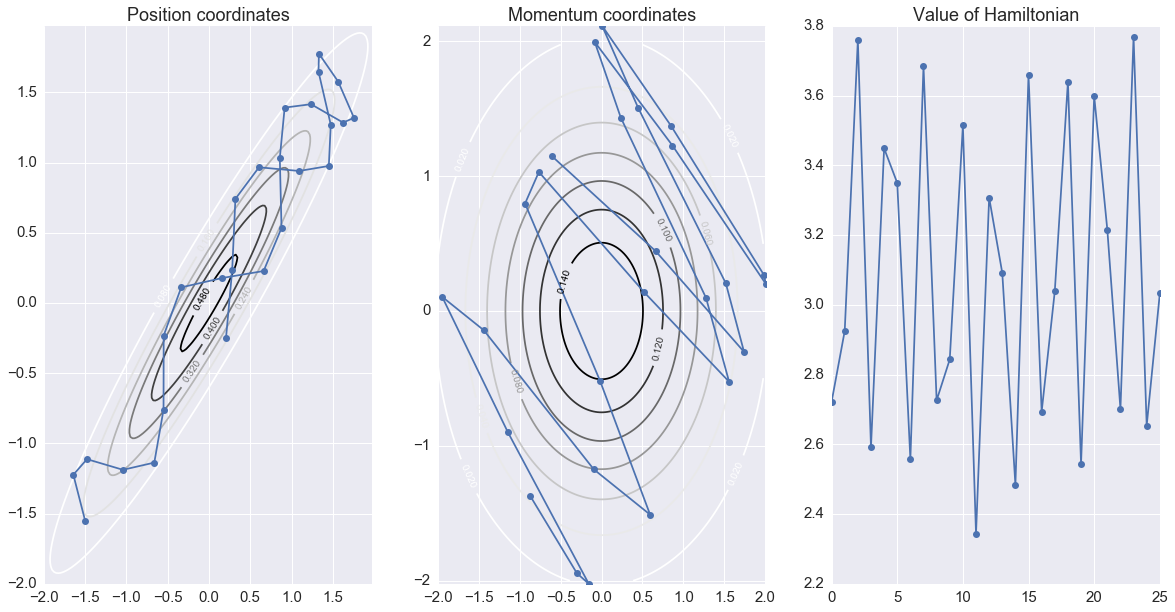
\includegraphics[width=1\linewidth]{HMC_eg.png}
  \caption{A trajectory for a 2D Gaussian distribution, simulated using 25 leapfrog steps with a stepsize of 0.25. The initial state for position variable q is $[-1.5,-1.55]^T$. Note how the position coordinate fully explores the space of the highly correlated distribution, while the momentum variables traverse the proposal space.}
\label{Fig:1}
\end{figure}


Note the differences between this and a random walk. The position variables move systematically throughout the space, reversing direction as dictated by the momentum coordinates so that the Hamiltonian oscillates appropriately. The small oscillations help the position variables fully explore the highly correlated space.\\

As in other methods, tuning HMC is important. Figure(\ref{Fig:2}) demonstrates what can happen when the step size is catastrophically large.
\begin{figure}[H]
\centering
  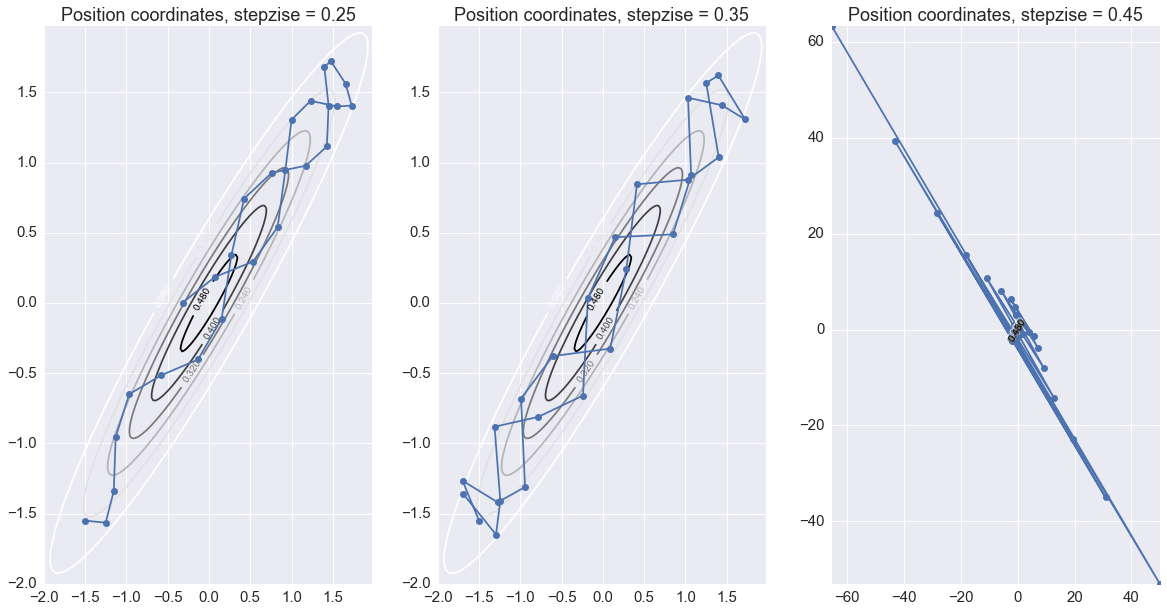
\includegraphics[width=1\linewidth]{HMC_critical_stepsize.png}
  \caption{Illustration of Hamiltonian trajectories with increasing stepsize until it reaches critical state.}
\label{Fig:2}
\end{figure}

The step size is mostly controlled by the need to keep the smaller steps ize under control. If larger step size were used the oscillation would be larger in the hamiltonian values. At a critical step size ($\epsilon =0.45$), the trajectory becomes unstable and the value of Hamiltonian grows without bound (figure \ref{Fig:2}). As long as the steps ize is less than that, the error in the hamiltonian stays bounded regardless of the number of leapfrog steps.


\subsection{Sampling from a two-dimensional distribution}
In this section we compare the trajectories between HMC and simple random-walk Metropolis method. The aim is to simulate from a bivariate Gaussian similar to the previous one but with stronger correlation of $0.98$. The HMC used the same kinetic energy as before. The results of $20$ HMC iteration with $L=20$ leapfrog steps with stepsize $\epsilon = 0.18$ are shown in the right of figure(\ref{Fig:3}). These values were chosen so that the trajectory length, $\epsilon L$, is sufficient to move to a distant point in the distribution without being so large that the trajectory will often back on itself. The rejection rate for this trajectories was $0.1$.
\begin{figure}[H]
\centering
  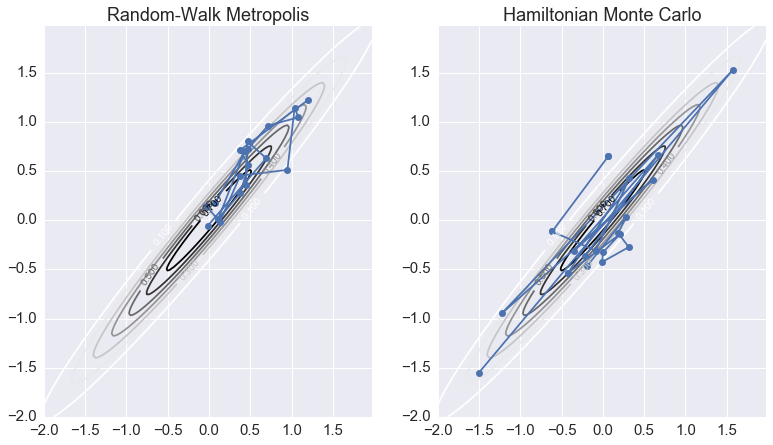
\includegraphics[width=1\linewidth]{MH_HMC_double_position.png}
  \caption{Twenty iterations from Metropolis (left) and HMC (right) sampling from bivariate Gaussians with .98 correlations.  The Metropolis method used a thinning of 20 iterations to compare to HMC with 20 steps per iterations, but HMC still explores the space much better.}
\label{Fig:3}
\end{figure}



Left image of the figure(\ref{Fig:3}) shows every 20th state from multiple iteration of random-walk Metropolis, with a bivaraite Gaussian proposal distribution (independent with standard deviations the same as step size for HMC, $\epsilon = 0.18$). The rejection rate for the random-walk proposals is $0.38$. Even with comparable steps, it is clear that HMC explores the target space much better than Metropolis, which is hampered by high correlation between the two variables.\\

Figure(\ref{Fig:4}) illustrates the result for $200$ HMC iterations and random-walk Metropolis iterations (thinned by 20 iterations). It is evident the autocorrelation between samples is much less in HMC and hence the state space is traversed more uniformly.


\begin{figure}[H]
\centering
  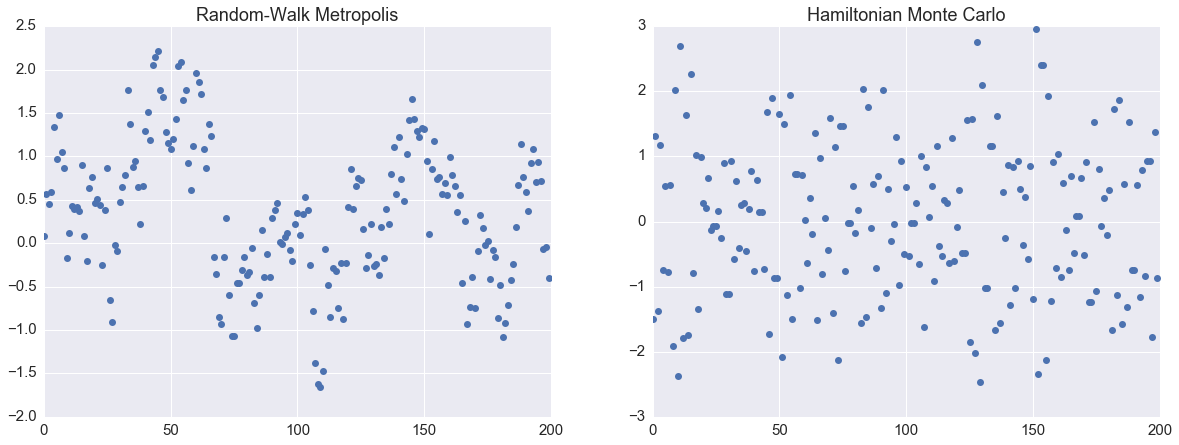
\includegraphics[width=1\linewidth]{MH_HMC_single_position.png}
  \caption{The first coordinate of the bivariate Gaussian sampled by the two methods. Metropolis (left) uses a thinning of 20 iterations to compare to HMC, which has 20 leapfrog steps per iteration. It is clear that there is high autocorrelation for Metropolis, even with this thinning, that is not apparent in HMC.}
\label{Fig:4}
\end{figure}

\subsection{Efficiency in High dimension}
In this section we show that HMC scales better than MH as a sampling algorithm. The target distribution to sample from is a $100$ dimensional Gaussian distribution, where the variables are independent, with means of zero, and standard deviations of $0.01,0.02,...,0.99,1.00$. We will use the same Kinetic energy function for the HMC as in the previous section, however it is $100$ dimensional instead of $2$.\\

For step size, we chose a number uniformly in $0.013 \pm 20\%$ - we chose a random number at each iteration in order to avoid situations where a leapfrog produces a full or half cycle of variables with standard deviations that are multiples of the step size. 0.013 was chosen to keep the step size on the same order as the smallest standard deviation of the target variables - in practice, we would not know this ahead of time, but diagnostics can be used to find the right value (selecting appropriate step sizes and number of leapfrog steps is not covered in this report). 150 leapfrog steps were used in order to allow the sampler to fully explore the space for the variables with larger standard deviations.\\

Figure(\ref{100d_iters}) shows the sample iterations for the last dimension (and thus largest standard deviation). To compensate for the 150 leapfrog steps, the Metropolis sampler thinned by 150 iterations.

\begin{figure}[H]
\centering
  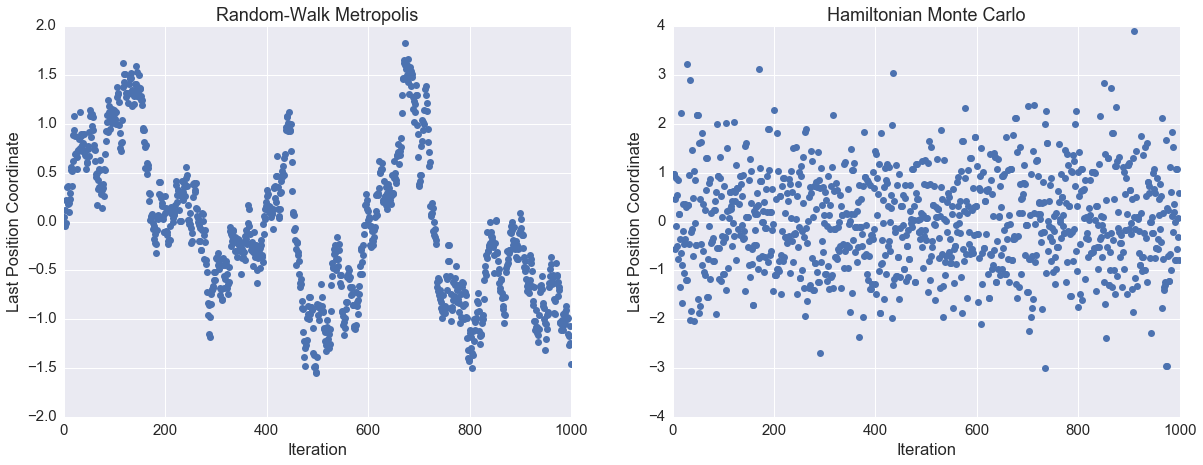
\includegraphics[width=1\linewidth]{100d_iterations.png}
  \caption{Iterations of sampled values for the last coordinate. The autocorrelation for random-walk Metropolis is even more pronounced.}
\label{100d_iters}
\end{figure}

Even when the target distributions have no correlations between variables, the high dimensionality causes the Metropolis sampler to be highly autocorrelated. Had the sampler not been thinned, the autocorrelation would have been even worse.\\

Perhaps more disturbing are the overall characteristics of the sampled distributions. We expect all sampled variables to have mean zero, and standard deviation to lie along the line y=x. Figures(\ref{100d_means}) and (\ref{100d_sds}) show the results for Metropolis and HMC.

\begin{figure}[H]
\centering
  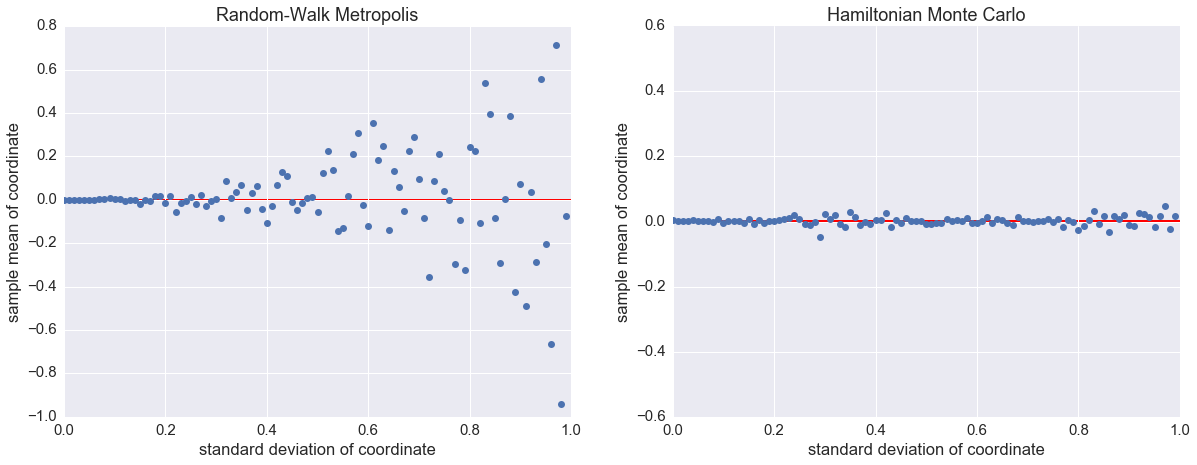
\includegraphics[width=1\linewidth]{100d_means.png}
  \caption{Sampled means for all 100 variables - we expect them all to be zero.}
\label{100d_means}
\end{figure}

\begin{figure}[H]
\centering
  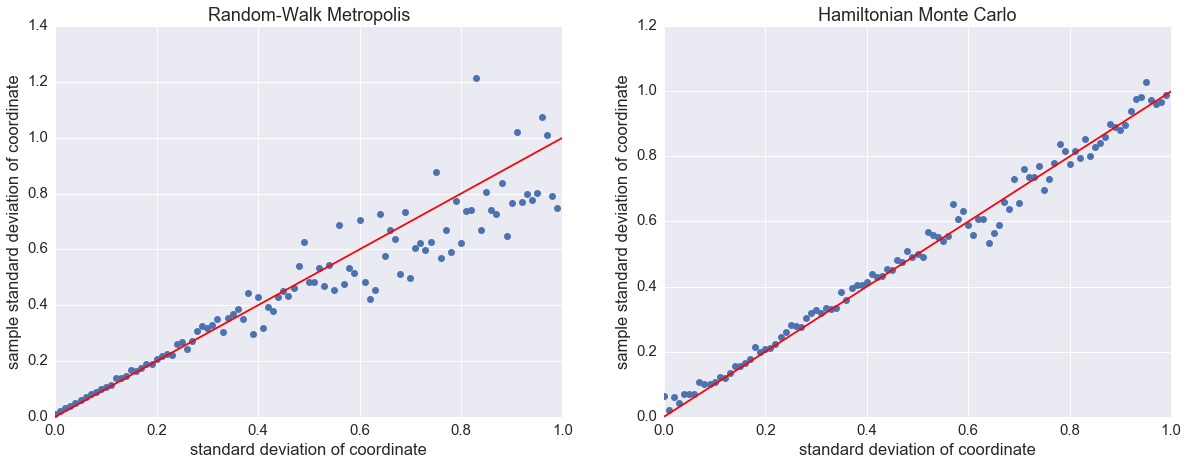
\includegraphics[width=1\linewidth]{100d_sds.png}
  \caption{Sampled standard deviations for all 100 variables - we expect them to lie along the line y=x.}
\label{100d_sds}
\end{figure}

Clearly, Metropolis fails us in the higher dimensions in this case. As the dimension increases (along with the standard deviations), the means fluctuate wildly. The standard deviations of the sampled values stray from their true values, and become more erratic in the higher dimensions. HMC shows neither of these traits - all the means are close to zero, and the sampled standard deviations lie close to the line y=x even in higher dimensions. Even with very simple, independent distributions, Metropolis fails in the larger dimensions where HMC succeeds  just as well as in the lower dimensions. 

\section{Windowed States}
For the final report, we plan on including a comparison to a modified version of HMC that helps obtain a higher probability of acceptance. This method, introduced by Neal in 1994, uses ``windows'' of states to probabilistically map the pair $(q,p)$ to a sequence of pairs, perform similar accept-reject steps, and then probabilistically map back. Following the 1994 paper, we will show improved efficiency of the algorithm.\\

The standard algorithm is as follows. For $1 \geq W \leq L + 1$ and $K$ randomly chosen from $\{0,...,W-1\}$, beginning at the initial state, perform $K$ leapfrog steps a random direction, and then $L - K$ from the initial state in the opposite direction. The reject window are the states from $-K$ to $-K + W - 1$, and the accept window are the states from $L-K-W+1$ to $L-K$. Note that each window is $W$ long and the whole leapfrog space is length $L$. The accept probability is the sum of the energy of the accept window divided by the sum of the energy of the reject window, chosen via a standard metropolis step. From the selected window, a specific state is then probability chosen with weight equal to its energy. Neal (1994) also offers a method which does not require a second pass through the chosen window. We apply that algorithm in our report - it is given explicitly below.\\

\textbf{Algorithm - Efficient Windowed States}
\begin{enumerate}
\item Begin with state $X_0$ (in our case $X_i = (q_i,p_i)$), stepsize $\epsilon$, leapfrog length $L$, window size $W$, offset $K$ randomly chosen from $\{0,...W-1\}$, and $\lambda$ randomly chosen from $\{-1,1\}$.\\
\item Perform $K$ leapfrog steps from $X_0$ with stepsize $\epsilon_R = -\lambda\epsilon$. These are states $\{X_{-1},...X_{-K}\}$.\\
\item Perform $L-K$ leapfrog steps from $X_0$ with stepsite $\epsilon_A = +\lambda\epsilon$. These are $\{X_1,...,X_{L-K}\}$.\\
\item Define the reject window $\mathcal{R}$ as $\{X_{-K},...,X_{-K+W-1}\}$ and the accept window $\mathcal{A}$ as $\{X_{L-K-W+1},...,X_{L-K}\}$.\\
\begin{enumerate}
\item Define $\mathcal{C}_{\mathcal{R}}^1 = X_{-K}$, `free energy' $\mathcal{F}_{\mathcal{R}}^1 = -H(X_{-K})$\\
\item While traversing the accept window via leapfrog steps, set $\mathcal{F}_{\mathcal{R}}^{i} = -\text{log}[\text{exp}(-H(X_{-K+i})) + \text{exp}(-\mathcal{F}_{\mathcal{R}}^{i-1}$)]. Set $\mathcal{C}_{\mathcal{R}}^{i} = \mathcal{C}_{\mathcal{R}}^{i-1}$ with probability exp$(-\mathcal{F}_{\mathcal{R}}^{i-1} + \mathcal{F}_{\mathcal{R}}^{i}$) and $\mathcal{C}_{\mathcal{R}}^{i} =  X_{-K+i}$ with probability exp$(-H(X_{-K+i}) + \mathcal{F}_{\mathcal{R}}^{i})$
\item Define $\mathcal{C}_{\mathcal{A}}^1 = X_{L-K-W+1}$, `free energy' $\mathcal{F}_{\mathcal{A}}^1 = -H(X_{-L-K-W+1})$\\
\item While traversing the reject window via leapfrog steps, set $\mathcal{F}_{\mathcal{A}}^{i} = -\text{log}[\text{exp}(-H(X_{-L-K-W+1+i})) + \text{exp}(-\mathcal{F}_{\mathcal{A}}^{i-1}$)]. Set $\mathcal{C}_{\mathcal{A}}^{i} = \mathcal{C}_{\mathcal{A}}^{i-1}$ with probability exp$(-\mathcal{F}_{\mathcal{A}}^{i-1} + \mathcal{F}_{\mathcal{A}}^{i}$) and $\mathcal{C}_{\mathcal{A}}^{i} =  X_{-L-K-W+1+i}$ with probability exp$(-H(X_{-L-K-W+1+i}) + \mathcal{F}_{\mathcal{A}}^{i})$
\end{enumerate}
\item Choose $C^{W}_{\mathcal{A}}$ with probability $-\text{log}\left(\frac{\sum_{X\in\mathcal{A}}\text{exp}(-H(X))}{\sum_{X\in\mathcal{R}}\text{exp}(-H(X))}\right)$ and $C^{W}_{\mathcal{R}}$ with 1 minus that probability.
\end{enumerate}

To demonstrate that this works as effectively as standard HMC, we plot the first 200 iterations with windowed HMC next to those from standard HMC. The target distribution was a bivariate Gaussian with standard deviations of one and covariances of 0.98.

\begin{figure}[H]
\centering
  \includegraphics[width=1\linewidth]{window_iter_2d}
  \caption{First 200 iterations of HMC (left) and windowed HMC (right) for bivariate Gaussian with standard deviations of 1 and covariance 0.98.}
\label{window_2d}
\end{figure}

As Figure~\ref{window_2d} shows, windowed HMC performs just as well as standard HMC with regards to exploring the space. Its value, however, is in the higher acceptance probability without sacrificing autocorrelation. To see this, we increase the dimensions to 10 and again compare to standard HMC.

\begin{figure}[H]
\centering
  \includegraphics[width=1\linewidth]{window_iter_10d}
  \caption{1000 iterations of HMC (left) and windowed HMC (right) for the last dimension of a 10-dimensional Gaussian with standard deviations ranging from 0.1 to 1.}
\label{window_10d}
\end{figure}

As we can see from Figure~\ref{window_10d}, again there is no loss in effective sample size with windowed HMC. The gain however, is in acceptance probability: we bump up from 87\% acceptance to 90\% acceptance. Though this may not seem like a significant increase, the difference becomes higher as dimension increases and the edge cases become more prevalent. For computational reasons, we do not perform higher dimensions.

\section{Parallelization}
We perform a trivial parallelization for MCMC. When sampling via MCMC, theory tells us that the chain will eventually converge to the target distribution. The standard method is to take a large burn-in, examine the trace plot, and look to see if convergence has occurred. If it has occurred, then each draw (if there is negligible autocorrelation, which is the case for HMC as we have seen) is an independent draw from the target distribution.  We can thus parallelize easily by running the chain separately, taking a burn-in in the hopes of convergence, and then pool the draws together. If there is no autocorrelation and the chains have converged, then we should be able to run them for a factor less than the number of chains running to get the same number of draws (i.e. if we run 4 chains, we should only have to run 4 times fewer iterations).\\

To demonstrate improvement in speed via parallelization, we ran 10 chains in the bivariate Gaussian case as before, with windowed HMC. We got a speedup factor of anywhere ranging from 1.3 to 2, which is not insignificant. In Figure~\ref{parallel} we plot every 100 iterations of the first 5 chains - we can see that even when starting in random places, the chains converge around the dense portion of the contour plot.

\begin{figure}[H]
\centering
  \includegraphics[width=1\linewidth]{WHMC_parallel.png}
  \caption{Every 100 iterations of windowed HMC on bivariate Gaussians with standard deviations of 1 and covariance of 0.98.  5 chains with random starting points are run}
\label{parallel}
\end{figure}


\section{Application to Real Data}
For our application to real data, we will demonstrate how the algorithm can be used to find the posterior values for parameters in simple linear regression. The model is as follows:

\begin{align*}
Y&\sim \mathcal{N}(X\beta, \phi^{-1}\mathcal{I})\\
\beta&\sim \mathcal{N}(0,\tau^{-1}\mathcal{I})\\
\phi&\sim \mathcal{G}(a,b)
\end{align*}

With hyperparameters $\tau,a,b$ = 0.1 to keep the priors for $\beta, \phi$ reasonably flat. We are most interested in the regression parameters $\beta$ - from frequentist statistics, we know that the least squares estimate $\hat{\beta} = (X^TX)^{-1}X^TY$. If our MCMC works correctly, it should produce a posterior value centered around $\hat{\beta}$ - we can use this as a test. Before we perform HMC, however, we need the potential energy $U(\theta)$ and its gradient. In our case, $\theta = [\phi, \beta]$, with $\beta$ $p$-dimensional. Recall that $U(\theta) = -\text{log}(p(\theta))$ - in our case, $p(\theta) \propto \pi(\theta)L(Y\mid\theta)$, the posterior of $\theta\mid Y$. The derivation of $U(\theta)$ is below.

\begin{align*}
\L(\theta\mid Y) &\propto L(Y\mid \phi,\beta)\pi(\beta)\pi(\phi)\\
&= \phi^{n/2}e^{-\frac{1}{2}\phi(Y-X\beta)^T(Y-X\beta)}e^{-\frac{1}{2}(\beta^T\tau\mathcal{I}\beta}\phi^{a-1}e^{-\phi b}\\
log(\theta\mid Y) &\propto (\frac{n}{2} + a - 1)\text{log}\phi - \frac{1}{2}\phi[\beta^TX^TX\beta - 2Y^TX\beta + Y^TY] - \frac{1}{2}\beta^T\tau\mathcal{I}\beta - \phi b\\
U(\theta) &= (-\frac{n}{2} - a + 1)\text{log}\phi + \phi b + \frac{1}{2}\{\beta^T[\phi X^TX + \tau\mathcal{I}]\beta - 2\phi Y^TX\beta\}
\end{align*}

From here we can get the partial derivatives
\begin{align*}
\frac{\partial U}{\partial \phi} &= \frac{-n - 2a + 2}{2\phi} + b\\
\frac{\partial U}{\partial \beta} &= \beta^T[\phi X^TX + \tau\mathcal{I}] - \phi Y^TX
\end{align*}
%\begin{comment}
\begin{thebibliography}{99} % Bibliography - this is intentionally simple in this template

\bibitem[1]NNeal, R., M.: MCMC using Hamiltonian dynamics 
\newblock arXiv:1206.1901v1 5(2)
(Jun 2012)
\bibitem[2]LLeimkuhler, B., Reikh, S.: Simulating Hamiltonian dynamics 
\newblock Cambridge University Press
(2004)
\end{thebibliography}
%\end{comment}



\end{document}
